\section{Kiến thức nền tảng}
Trước khi đi vào nghiên cứu bài đề cương luận văn này, một số kiến thức nền tảng cần được nhắc lại như sau.
\subsection{Các kiến thức toán cơ bản}
%TODO: Ma trận, phép nhân covl, phép nhân element-wise, phép đạo hàm,.. 
\textbf{Phép nhân tích chập ma trận (convolution)}

Nhân tích chập là phép toán quan trọng trong Xử lý ảnh số và thị giác máy tính, là công cụ chủ yếu để thực hiện
các phép tính toán trên ảnh như đạo hàm ảnh, làm trơn ảnh hay trích xuất cạnh.

Trong toán học, tích chập là phép toán trên hai hàm f và g, tạo ra hàm thứ ba là hàm (f*g). Công thức phép tích
chập trên miền liên tục một chiều như sau:

$(f*g)(t) \triangleq \displaystyle \int_{-\infty}^{\infty}f(\tau)g(t-\tau)d\tau$


Đối với trong Xử  lý ảnh, phép tích chập được tính trên miền không gian hai chiều, rời rạc. Công thức tính tích
chập trên ảnh f và bộ lọc k (kích thước mxn) tại điểm ảnh vị trí (x,y) với giả sử chỉ số trên bộ lọc được đánh số hàng từ -m/2 -> m/2
và chỉ số cột từ -n/2 -> n/2:

$(k*f)(x,y) \triangleq \displaystyle \sum_{u=-m/2}^{m/2}\displaystyle \sum_{v=-n/2}^{n/2}k(u,v)f(x-u,y-v)$

Một phép toán tương tự covolution nhưng không xoay bộ lọc như trên, gọi là correlation (hình 1), công thức như sau:

$(k*f)(x,y) \triangleq \displaystyle \sum_{u=-m/2}^{m/2}\displaystyle \sum_{v=-n/2}^{n/2}k(u,v)f(x+u,y+v)$
\begin{figure}[!h]
    \begin{center}
        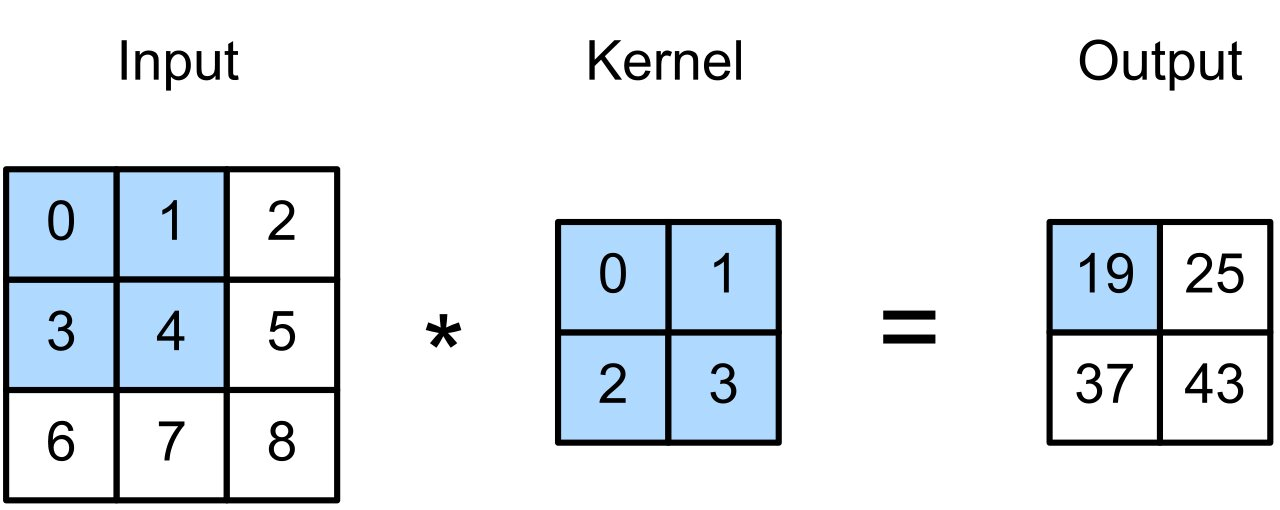
\includegraphics[width=\linewidth]{asset/image/correlation.jpg}
        \caption{Phép correlation.}
    \end{center}
\end{figure}


%chưa nhắc tới strike hay padding gì cả


\subsection{Các kiến thức cơ bản về  Trí tuệ nhân tạo, học máy và học sâu}
\subsubsection{Các kiến thức cơ bản}
%TODO: gradient descent, overfit, underfit, hội tụ, bias, variant, weight, model, loss function, .. tham khảo machinelearningcoban để tránh thiếu sót
\textbf{Gradient descent - back propagation}

\textbf{Overfitting}

\textbf{Hội tụ}

\textbf{Variance - bias}

\textbf{Objective function - loss function}
\textbf{}
\textbf{}
\textbf{}
\textbf{}
\textbf{}

\subsubsection{Phân loại các phương pháp học}
\textbf{Phân loại phương pháp học}
%TODO: hiện nay có 4 loại học phổ biến: supervised, unsupervised, reinforcement learning, và các phương pháp kết hợp (semi-supervised learning)
\textbf{Phân loại theo ứng dụng}

